\chapter{Resultados y discusión}

\section{Estabilidad de estructuras}

Se estudian los posibles isómeros conformacionales de los ácidos sulfúrico, carbónico y fosfórico (ANEXO) con el fin de hallar la estructura más estable en fase gas. \\

  \begin{table}[H]
\begin{center}
\begin{tabular}{|c|c|c|c|c|c|}
\hline
Isómeros $H_2SO_4$ & $\Delta E$ & Isómeros $H_2CO_3$ & $\Delta E$ & Isómeros $H_3PO_4$ & $\Delta E$ \\ \hline
$Conf_1$ & 4,1908 & $Conf_1$ & 0,0000 & $Conf_1$ & 0,9832 \\ \hline
$Conf_2$1 & 2,5058 & $Conf_2$1 & 1,3775 & $Conf_2$ & 0,4458 \\ \hline
$Conf_3$2 & 0,0000 & -- & -- & $Conf_3$ & 0,0000 \\ \hline
-- & -- & -- & -- & $Conf_4$ & 0,6187 \\ \hline
\end{tabular}
\caption{Diferencias de la energía libre de Gibbs en Kcal/mol de cada isómero conformacional de los ácidos a estudiar}
\label{tab:3.1}
\end{center}
\end{table}
A la vista de los resultados de energías expuestos en la Tabla 3.1, el isómero más estable del ácido sulfúrico es el confórmero 3, debido a que dicha disposición espacial minimiza las repulsiones de los pares de electrones originando una baja energía y a su vez una mayor estabilidad, ésta también se debe a la posible formación de puentes de hidrógeno intramoleculares, ya que los hidrógenos 3 y 7 de dicho confórmero están dirigidos hacia los átomos de oxígeno 5 y 4 respectivamente, con dos pares de electrones libres en orbitales p, la distancia de los H a los O es menor que la suma de sus radios de Van Der Waals (Tabla 3.2), los H presentan una carga positiva y los oxígenos una negativa como se muestra en la figura 3.1.
	\begin{table}[H]
\begin{center}
\begin{tabular}{|c|c|}
	\hline
	\multicolumn{2}{|c|}{Radio de Van Der Waals en $\Armstrong$} \\ \hline
	O & 1,5 \\ \hline
	H & 1,2 \\ \hline
\end{tabular}
\caption{Valor de los radios de Van Der Waals en $\Armstrong$}
\end{center}	
\end{table}
\begin{figure}[H]
	\centering
	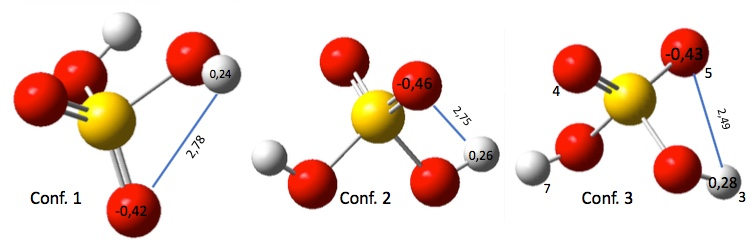
\includegraphics[scale=0.4]{prezimagen}
	\caption{Parámetros para un enlace de hidrógeno, distancias en $\Armstrong$}
\end{figure}

El isómero del ácido carbónico más estable es el $H_2CO_3$, pero hay que tener en cuenta que la diferencia de energía es mínima, los dos isómeros presentan una estructura trigonal plana, y un enlace muy fuerte CO, pero dicho confórmero posee una de las otras dos distancias CO menor que en el $H_2CO_3$1, Tabla 3.3, por tanto sus enlaces son más fuertes y la molécula presenta menor energía total y mayor estabilidad, tabla \ref{tab:3.1}. 
\begin{table}[H]
    \centering
    \begin{tabular}{|c|c|c|}
    \hline
    Ácido & $d(C-OH_{(1)})$ & $d(C-OH_{(2)})$ \\ \hline
    $H_2CO_3$ & 1,34 & 1,34  \\ \hline
    $H_2CO_3$1 & 1,36 & 1,34 \\ \hline 
    \end{tabular}
    \caption{Distancias C-OH del ácido carbónico}
\end{table}

En cuanto a los isómeros del ácido fosfórico, no se puede decir que el $H_3PO_4$2 sea el más estable ya que las diferencias de energía son demasiado pequeñas, y entra dentro del error que puede tener el software utilizado. Ver tabla \ref{tab:3.1}

Se estudia también la estabilidad de los confórmeros de los ácidos anteriores sustituyendo uno o varios átomos de hidrógeno por halógenos. Tablas de la 3.4 a la 3.7.

En primer lugar se estudian los confórmeros del ácido sulfúrico sustituido, donde el $HClSO_4$1 tiene dos enlace S-O muy fuerte (d(S-O)=1,43$\Armstrong$) y la disposición del cloro es tal que no hay impedimento estérico ya que está en trans con el hidrógeno. (Ver Fig:3.2). El $SO_4HF$ es la molécula más estable en la sustitución de un hidrógeno por un átomo de flúor, ya que es la única con dos enlaces S-O muy fuertes (d(S-O)=1,43 $\Armstrong$), esto es porque el flúor esta a una distancia muy grande (d(S-F)=2,52$\Armstrong$) y permite la fortaleza de los demás enlaces.

\begin{table}[H]
	\begin{center}
		\begin{tabular}{|c|c|c|c|}
			\hline
			Sustitución por F & $\Delta E$ & Sustitución por Cl & $\Delta E$ \\ \hline
			$HFSO_4$	& 10,818 & $HClSO_4$ & 0,0555 \\ \hline
			$HFSO_4$1 & 10,777 & $HClSO_4$1 & 0,0000 \\ \hline
			$HFSO_4$2 & 10,780 & $HClSO_4$2 & 65,028 \\ \hline
			$HFSO_4$3 & 10,826 & $HClSO_4$3 & 64,227 \\ \hline
			$HFSO_4$4 & 42,675 & $HClSO_4$4 & 24,428 \\ \hline
			$HFSO_4$5 & 10,826 & $HClSO_4$5 & 0,0427 \\ \hline
			$HSO_4F$ &	101,31 & $HSO_4Cl$ & 109,95 \\ \hline
			$SO_4HF$ &	0,0000 & $SO_4HCl$ & 4,8299 \\ \hline
		\end{tabular}
		\caption{Diferencias de la energía libre de Gibbs en Kcal/mol de cada isómero conformacional del ácido sulfurico sustituyendo un H por un halógeno}
	\end{center}
\end{table}

Los confórmeros más estables del ácido carbónico sustituido con halógenos presentan distancias menores de enlaces C-O, es decir, enlaces más fuertes, por lo que poseen una energía total menor.

\begin{table}[H]
	\begin{center}
		\begin{tabular}{|c|c|c|c|}
			\hline 
			Sustitución por F & $\Delta E$ & Sustitución por Cl & $\Delta E$ \\ \hline
			$HFCO_3$1 & 3,9632 & $HClCO_3$ & 48,952 \\ \hline
			$HFCO_3$ & 3,8449 & $HClCO_3$1 & 49,890 \\ \hline
			$HCO_3F$ & 92,693 & $HCO_3Cl$ & 91,991 \\ \hline
			$CO_3HF$ & 1,8115 & $CO_3HCl$ & 0,0000 \\ \hline
			$CO_3HF$1 & 0,0000 & $CO_3HCl$1 & 0,3151 \\ \hline
		\end{tabular}
		\caption{Diferencias de la energía libre de Gibbs en Kcal/mol de cada isómero conformacional del ácido carbónico sustituyendo un H por un halógeno}
	\end{center}
\end{table}

{\bfseries\textcolor{red} {AQUI NO SE SI PONER TABLA CON LAS DISTANCIAS C-O DE CADA MOLECULA, PORQUE YA SON MUCHAS TABLAS, PUEDO HACERLA Y PONERLA EN EL ANEXO Y REFERENCIARLA: "....energía total menor", ver tabla: anexo X.}}

Análogamente a lo dicho en los casos de los ácidos anteriores se concluye que los compuestos más estables al sustituir un hidrógeno por un halógeno en el caso del ácido fosfórico son el $H_2FPO_4$8 y el $H_2ClPO_4$2. y al sustituir un hidrógeno más por otro halógeno las moléculas de mayor estabilidad son el $HF_2PO_4$ y el $PO_4HCl_2$ 

\begin{table}[H]
\begin{center}
\begin{tabular}{|c|c|c|c|}
\hline
Sustitución por F & $\Delta E$ & Sustitución por Cl & $\Delta E$ \\ \hline
$H_2FPO_4$& 1,2641 & $H_2ClPO_4$ & 0,8643 \\ \hline
$H_2FPO_4$1 & 1,2640 & $H_2ClPO_4$1 & 0,8675 \\ \hline
$H_2FPO_4$2 & 0,0014 & $H_2ClPO_4$2 & 0,0000 \\ \hline
$H_2FPO_4$4	& 8,6205 & $H_2ClPO_4$3 & 40,005 \\ \hline
$H_2FPO_4$3	& 8,6218 & $H_2ClPO_4$4 & 40,001 \\ \hline
$H_2FPO_4$5	& 56,668 & $H_2ClPO_4$5 & 29,134 \\ \hline
$H_2FPO_4$6	& 8,4010 & $H_2ClPO_4$6 & 40,725 \\ \hline
$H_2FPO_4$7	& 8,6178 & $H_2ClPO_4$7 & 43,487 \\ \hline
$H_2FPO_4$8	& 0,0000 & $H_2ClPO_4$8 & 29,959 \\ \hline
$H_2FPO_4$9	& 57,869 & $H_2ClPO_4$9 & 90,161 \\ \hline
$H_2PO_4F$ & 22,242 & $H_2PO_4Cl$ & 1,2929 \\ \hline
$PO_4H_2F$ & 23,164 & $PO_4H_2Cl$ & 0,5166 \\ \hline
\end{tabular}
\caption{Diferencias de la energía libre de Gibbs en Kcal/mol de cada isómero conformacional del ácido fosfórico sustituyendo un hidrógeno por un halógeno.}
\end{center}
\end{table}

\begin{table}[H]
	\centering
	\begin{tabular}{|c|c|c|c|}
		\hline
		Sustitución por 2 átomos F & $\Delta E$   & Sustitución por dos átomos Cl & $\Delta E$     \\ \hline
		$HF_2PO_4$  & 0,000     & $HCl_2PO_4$     & 98,649 \\ \hline
		$HF_2PO_4$1  & 18,038    & $HCl_2PO_4$1   & 38,457 \\ \hline
		$HF_2PO_4$2   & \#¡VALOR! & $HCl_2PO_4$2    & 39,297 \\ \hline
		$HF_2PO_4$3   & \#¡VALOR! & $HCl_2PO_4$3    & 39,330 \\ \hline
		$HF_2PO_4$4   & \#¡VALOR! & $HCl_2PO_4$4  & 38,462 \\ \hline
		$PO_4HF_2$    & 60,559    & $PO_4HCl_2$  & 0,000  \\ \hline
		$PO_4HF_2$1   & 60,559    & $PO_4HCl_2$1   & 2,077  \\ \hline
		$FPO_4HF$    & 15,887    & $ClPO_4HCl$  & 19,523 \\ \hline
		$FPO_4HF$1   & 36,514    & $ClPO_4HCl$1   & 0,101  \\ \hline
		$FPO_4HF$2  & 39,126    & $ClPO_4HCl$2   & 38,645 \\ \hline
	\end{tabular}
\caption{Diferencias de la energía libre de Gibbs en Kcal/mol de cada isómero conformacional del ácido fosfórico sustituyendo dos hidrógenos por dos halógenos.}
\end{table}

También se ha realizado el estudio de estabilidad de dichos ácidos frente a la sustitución de hidrógenos por diferentes halógenos. Ver figura 3.2. \\
En la tabla 3.8 se observa la diferencia de energía, entre los ácidos sustituidos por flúor o cloro y los no sustituidos.


\begin{table}[H]
	\centering
	\begin{tabular}{|c|c|c|c|c|c|}
		\hline
		Ácido	& $\Delta E$ &	Ácido	& $\Delta E$ & Ácido & $\Delta E$\\ \hline
		$ H_2SO_4$	& 0	& $H_2CO_3$	 & 0 &	$H_3PO_4$	& 0 \\ \hline
		$HFSO_4$ &	6,22E+04	& $HFCO_3$	& 6,22E+04	& $H_2ClPO_4$	& 2,88E+05 \\ \hline
		$HClSO_4$ &	2 ,88E+05	& $HClCO_3$ &	2,88E+05	& $HCl_2PO_4$ &	5,77E+05 \\ \hline
	\end{tabular}
	\caption{Diferencias de energía en Kcal/mol}
\end{table}

\begin{figure}[H]
	\centering
	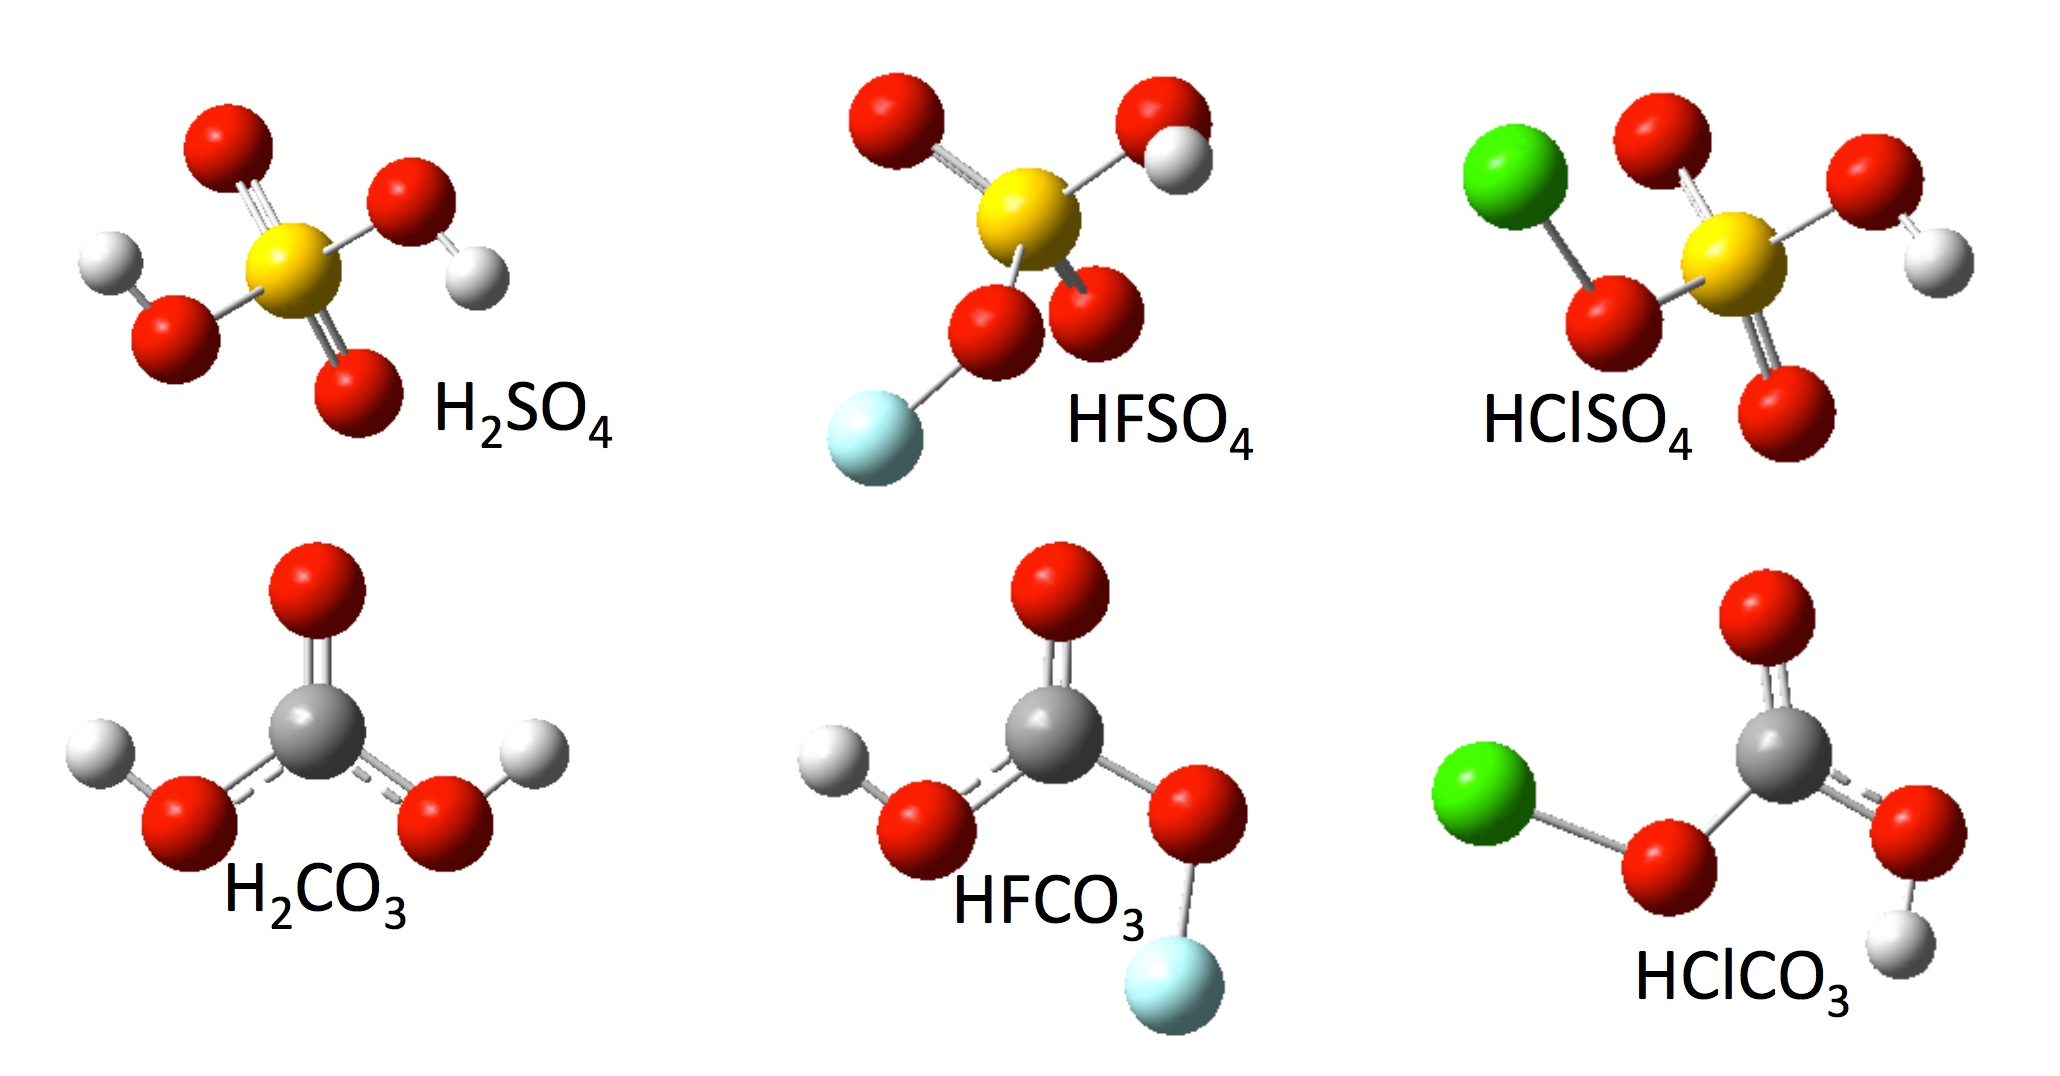
\includegraphics[scale=0.15]{ESH}
	\caption{Sustitución de hidrógenos por diferentes halógenos}
\end{figure}


La estabilidad de la molécula aumenta con la sustitución del halógeno, esto se debe a su efecto inductivo (electronegatividad), por otro lado, aunque el flúor sea más electronegativo que el cloro (3,98 y 3,16 respectivamente), la estabilidad aumenta al sustituir un hidrógeno por este último halógeno por su mayor tamaño, ya que cuanto más espacio se tenga, más ``cómodo'' estará el electrón y más estable será la molécula.
También se observa como la estabilidad aumenta al aumentar el número de sustituciones de hidrógeno por el halógeno, ver columnas 5 y 6 de la tabla 3.8, por el efecto inductivo del halógeno mencionado antes.



\begin{figure}[h]
	\centering
	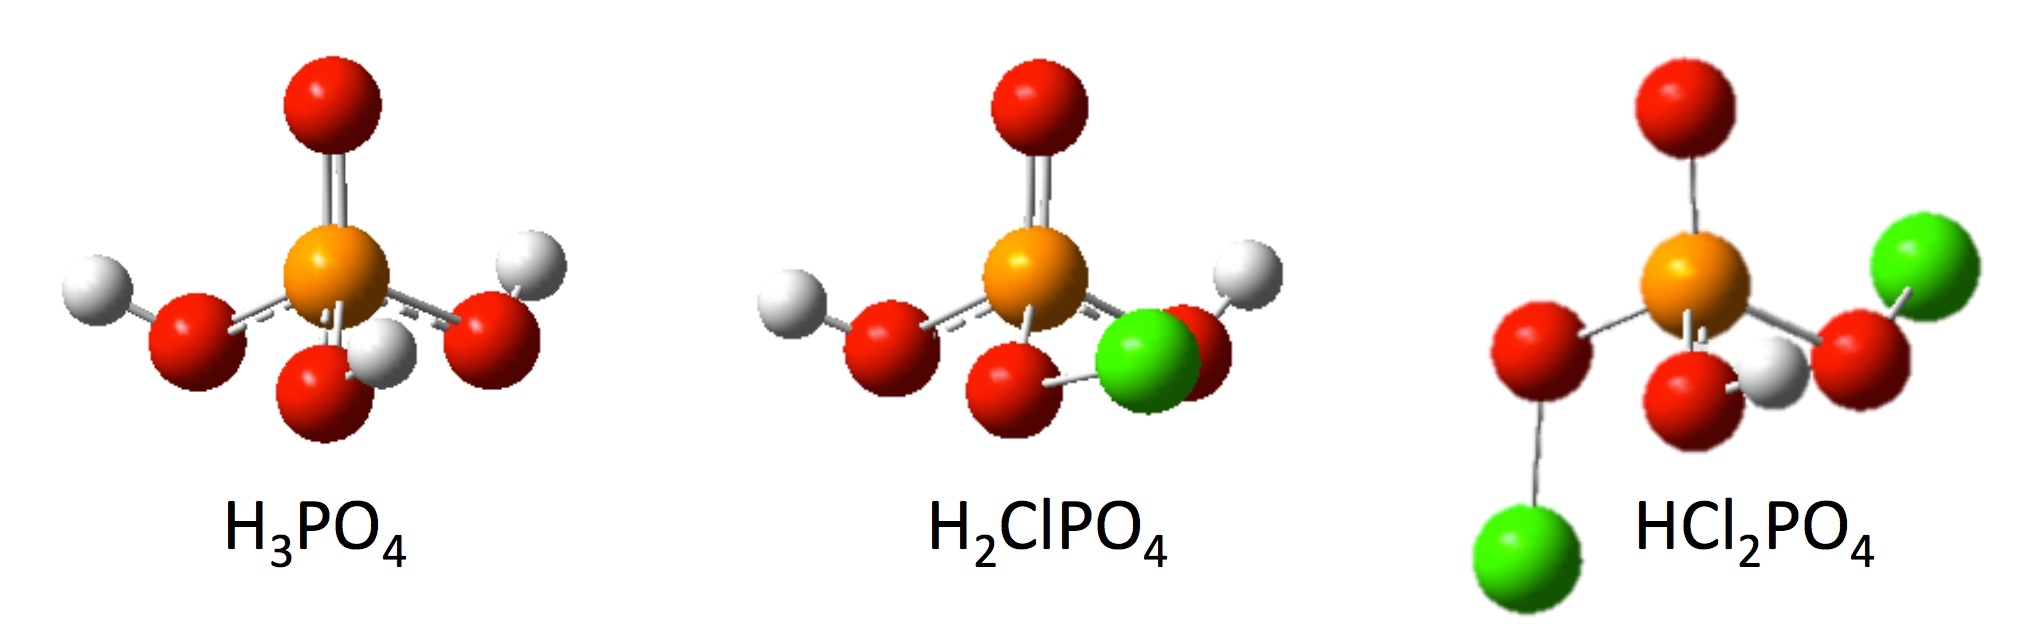
\includegraphics[scale=0.15]{ESH2}
	\caption{Sustitución de hidrógenos por más de un halógeno }
\end{figure}

\section{Acidez en fase gas de moléculas}

Con el fin de estudiar el impacto de estas sustituciones en la acidez en fase gas de los ácidos, se han diseñado más estructuras sustituyendo hidrógenos por fluor. Para calcular la acidez en fase gas se han hecho los mismos cálculos computacionales con sus aniones.
También se ha sustituido el grupo ácido por otro para así ver el cambio de acidez en fase gas.

 \begin{table}[H]
     \centering
     \begin{tabular}{|c|c|c|c|}
     \hline
     \multicolumn{4}{|c|}{\bfseries{ACIDEZ}} \\ \hline
     Ácido & $\Delta G$ & $\Delta G_{exp}$ & $\Delta G_{ H. especf}$ \\ \hline
$CF_3COOH$ & 314,04 & 316,3 & 309,0282809\\ \hline
$CF_3COSH$ & 311,58 & 312,5 & 303,3527667\\ \hline
$CF_3SO_3H$ & 292,87 & 299,5 &292,2881339\\ \hline
$FHSO_3$ & 293,57 & 299,8 & 293,0524411\\ \hline
$H_2CFCOOH$ & 328,14 &-- & 320,5998791\\ \hline
$H_2CFCOSH$ & 323,99 & --& 314,4709262\\ \hline
$H_2CFSO_3H$ & 303,60 & -- & 302,9127567\\ \hline
$H_2CO_3$ & 327,95	& -- & 319,6992767\\ \hline
$H_2S_2O_6$ & 281,75 & -- & 283,4104362\\ \hline
$H_2SO_4$ & 302,60	& 302,2 & 301,2892628\\ \hline
$H_3CCOOH$ & 338,57 & -- &	328,9212264\\ \hline
$H_3CCOSH$ & 330,46 & -- &	319,4866136\\ \hline
$H_3CSO_3H$ & 312,65 & 315,0 & 309,7167849\\ \hline
$HCF_2COOH$ & 	321,43 & -- & 314,9858609\\ \hline
$HCF_2COSH$ & 	316,83 & -- & 308,5712026\\ \hline
$HCF_2SO_3H$ & 	297,86 & -- & 298,3781185\\ \hline
$HPO_3$ & 303,54 & 303,3 & 300,9305154\\ \hline
$HNO_3$ & 315,01 & 317,8 & 309,4734993\\ \hline
$H_3PO_4$ & 321,44	& -- & 332,5547603 \\ \hline
     \end{tabular}
     \caption{Acideces en fase gas con y sin hidratación específica y el valor experimental en Kcal/mol. $\cite{quimica3}$ }
     \label{tab:3.9}
 \end{table}
 
 Los resultados dados en la Tabla 3.9 apoyan el siguiente orden de acidez intrínseca para los ácidos orgánicos: $ CF_3SO_3H>HCF_2SO_3H>H_2CFSO_3H>CF_3COSH>H_3CSO_3H>CF_3COOH>HCF_2COSH>HCF_2COOH>H_2CFCOSH>H_2CFCOOH>H_3CCOSH>H_3COOH $, y el siguiente para los oxácidos: $ H_2S_2O_6>FHSO_3>H_2SO_4>HPO_3>HNO_3>H_3PO_4>H_2CO_3 $.

Los ácidos llamados normalmente fuertes ($ CF_3SO_3H$, $FHSO_3$, $HCF_2SO_3H$, $H_2SO_4$, $HPO_3$, $H_2CFSO_3H$) están en un intervalo de acidez relativamente estrecho (10,7 kcal/mol), se tienen algunos valores experimentales, donde la variación con los calculados computacionalmente no llega a las 3 Kcal/mol exceptuando al $CF_3SO_3H$ y al $FHSO_3$ que difieren de 6-7 kcal/mol, al tener una diferencia tan alta, se ha llevado a cabo un cálculo G4 para estos dos últimos ácidos con el fin de ver si el primer cálculo sobreestima la acidez de dichos ácidos. 
\begin{table}[H]
	\centering
	\begin{tabular}{|c|c|c|}
		\hline
		Ácido & $\Delta G$ & $\Delta G_{exp}$ \\ \hline
		$CF_3SO_3H$ &{\bfseries dato }& 299,5 \\ \hline
		$FHSO_3$ & {\bfseries dato } & 299,8 \\ \hline 
	\end{tabular}
\caption{Acideces en fase gas con el método G4 en Kcal/mol}
\end{table}

La acidez es proporcional a la tendencia del ácido a perder un protón. Se ve como el orden de acidez sustituyendo el grupo ácido es $ COOH {<} COSH {<} SO3H $, ya que en los aniones correspondientes se debe tener en cuenta la estabilización por resonancia, deslocalización de enlaces $\pi$, que es mayor en el $SO3^-$ ya que hay mayor número de átomos, en cuanto a las otras dos estructuras, los iones $COS^-$ y $COO^-$ son estabilizados por resonancia, pero en el $COS^-$ es mayor, se puede explicar observando la carga Mulliken en dichos átomos dada en la tabla 3.11. Ver figura 3.4.

\begin{figure}[H]
	\centering
	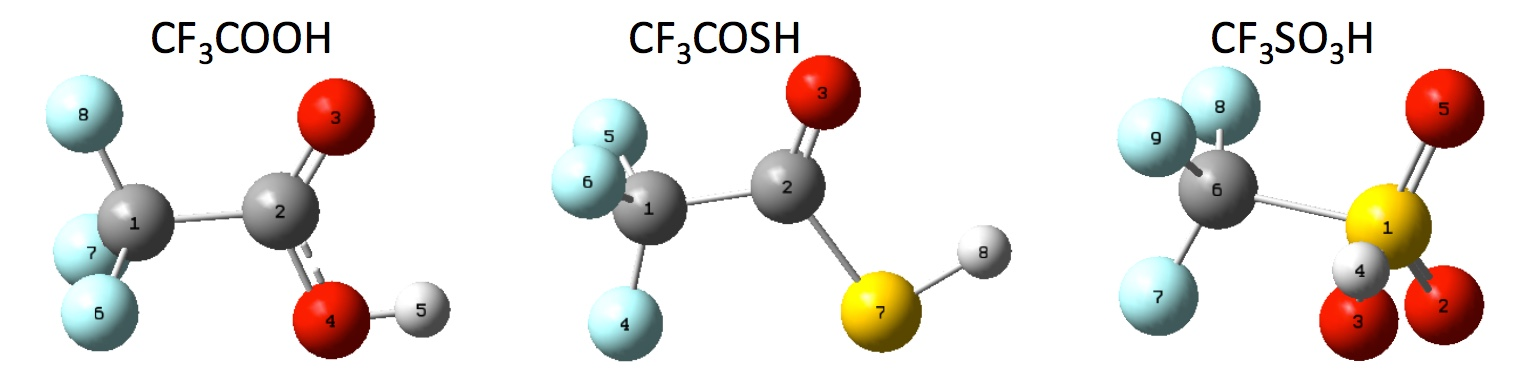
\includegraphics[scale=0.2]{CF3-grupo}
	\caption{Ácidos con tres átomos de flúor}
\end{figure}

\begin{table}[H]
    \centering
    \begin{tabular}{|c|c|c|c|c|c|}
    \hline
    $SO3^-$ & Carga Mulliken &$COS^-$ & Carga Mulliken & $COO^-$ & Carga Mulliken \\ \hline
    S & 1.007134 & S & -0.503466 & C & 0.201081 \\ \hline
    O & -0.575748 & O & -0.381057 & O & -0.482870 \\ \hline
    O & -0.575646 & C & -0.018142 & O & -0.491545 \\ \hline
    O & -0.575761 & -- & -- & -- & -- \\ \hline
    \end{tabular}
    \caption{Carga Mulliken de la moléculas $CF_3-$ grupo ácido}
\end{table}

Comparamos también sustitución de átomos de flúor por átomos de hidrógeno en el grupo $CF_3$ de la molécula. En la tabla \ref{tab:3.9} se ve que cuantos más átomos de flúor haya en la molécula mayor es su acidez, esto se debe a la elevada electronegatividad del flúor, cuántos más átomos de flúor haya, mayor capacidad atractora tendrá el grupo, y mayor será el efecto inductivo, polarización de carga transmitida por enlaces $\sigma$, si se observa la carga Mulliken (tabla 3.12) en los átomos de las moléculas se comprueba su estabilización por resonancia. Ver figura 3.5.

\begin{figure}[H]
	\centering
	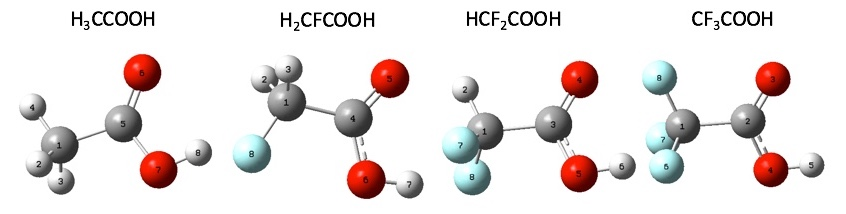
\includegraphics[scale=0.4]{grupo-COOH}
	\caption{Ácidos carboxílicos con diferentes sustituciones de hidrógenos por átomos de flúor.}
\end{figure}
\begin{table}[H]
    \centering
    \begin{tabular}{|c|c|c|c|c|c|c|c|}
    \hline
    $CF_3-$ & Carga Mull & $HCF_2-$ & Carga Mull & $H_2CF-$ & Carga Mull & $H_3C-$ & Carga Mull \\ \hline
     C & 0.549474 &  C & 0.382878 & C & 0.151906 & C & -0.189412 \\ \hline
     C & 0.201081 &  C & 0.204525 & C & 0.203532 & C & 0.234883 \\ \hline
     O & -0.482870 & O & -0.510709 & O & -0.527054 & O & -0.519973 \\ \hline
     O & -0.491545 & O & -0.488498 &  O & -0.493739 & O & -0.525498 \\ \hline
     F & -0.261497 & F & -0.287967 & F & -0.334645 &  & \\ \hline
     F & -0.261531 & F & -0.300230 &  &  &  & \\ \hline
     F & -0.253112 &  &  &  &  &  & \\ \hline
    \end{tabular}
    \caption{Carga Mulliken de moléculas grupo-COOH con las cargas de hidrógenos sumadas dentro de los átomos pesados.}
\end{table}

\subsection{Hidratación específica}
Se estudia el impacto que tiene la hidratación específica en la acidez de las moléculas anteriores, en la tabla \ref{tab:3.9} también se indica la acidez en presencia de una molécula de agua en fase gas.
A la vista de los resultados expuestos, la acidez aumenta al haber una molécula de agua en un punto determinado de la molécula, ya que se forman enlaces de hidrógeno fuertes como se puede comprobar mirando las distancias d(O-H) y teniendo en cuenta la existencia de un máximo de densidad en dichos enlaces en la tabla 3.13. 

{\bfseries TENGO QUE MIRAR DETENIDAMENTE EL H3PO4 Y H3PO4-H2O}

\begin{table}[H]
	\centering
	\begin{tabular}{|c|c|c|c|}
		\hline
		Ácidos-$H_2O$ & distancia	& d(O-H) ($\Armstrong$) & $Max_{densidad}$ \\ \hline
		$CF_3COOH-H_2O$ & $d(O_9-H_5)$ &1,6926&4,665E-02\\ \cline{2-4}
& $d(O_3-H_{10})$ & 2,1371 & 1,852E-02 \\ \hline
 $CF_3COSH-H_2O$ & $d(O_9-H_8)$	 & 1,9225 & 3,014E-02 \\ \cline{2-4}
	& $d(O_3-H_{10})$ & 2,0486 & 2,064E-02 \\ \hline
	$CF_3SO_3H-H_2O$ & $d(O_{10}-H_4)$ & 1,6142 & 5,653E-02 \\ \cline{2-4}
	& $d(O_5-H_{12})$	& 2,1910 &	1,631E-02 \\ \hline
 $FHSO_3-H_2O$	& $d(O_7-H_4)$ & 1,6098 &	5,682E-02 \\ \cline{2-4}
	& $d(O_5-H_8)$	& 2,3134	& 1,323E-02 \\ \hline
 $H_2CFCOOH-H_2O$	&$d(O_9-H_7)$ & 1,7347	& 4,251E-02 \\ \cline{2-4}
	& $d(O_5-H_{11})$ & 2,0119	& 2,375E-02 \\ \hline
 $H_2CFCOSH-H_2O$ &	$d(O_3-H_{10})$ & 1,9847 &	2,356E-02 \\ \cline{2-4}
	& $d(O_9-H_6)$ & 1,9897	& 2,633E-02 \\ \hline
 $H_2CFSO_3H-H_2O$ &	$d(O_{10}-H_4)$	& 1,6489	& 5,205E-02 \\ \cline{2-4}
	& $d(O_5-H_{11})$ & 2,0786	& 2,015E-02 \\ \hline
 $H_2CO_3-H_2O$	& $d(O_7-H_5)$	& 1,7367	& 4,163E-02 \\ \cline{2-4}
	& $d(O_2-H_9)$ & 2,2011	& 1,575E-02 \\ \hline
 $H_2S_2O_6-H_2O$ &	$d(O_{11}-H_{10})$	& 1,5480 &	6,753E-02 \\ \cline{2-4}
	& $d(O_2-H_{12})$ & 2,0478 &	1,959E-02 \\ \hline
 $H_2SO_4-H_2O$	& $d(O_8-H_5)$ & 1,6514	& 5,181E-02 \\ \cline{2-4}
	& $d(O_6-H_9)$ & 2,1459	& 1,768E-02 \\ \hline
 $H_3CCOOH-H_2O$ & $d(O_9-H_8)$ & 1,7673	& 3,947E-02 \\ \cline{2-4}
	& $d(O_6-H_{10})$ & 1,9607 &	2,645E-02 \\ \hline
 $H_3CCOSH-H_2O$ &	$d(O_3-H_{10})$	& 1,9582 &	2,496E-02 \\ \cline{2-4}
	& $d(O_9-H_5)$	& 1,9999	& 2,587E-02 \\ \hline
 $H_3CSO_3H-H_2O$	& $d(O_{10}-H_4)$	& 1,6892	& 4,736E-02 \\ \cline{2-4}
	& $d(O_5-H_{11})$	& 2,0648 &	2,080E-02 \\ \hline
 $HCF_2COOH-H_2O$	& $d(O_9-H_6)$	&1,7146	& 4,446E-02 \\ \cline{2-4}
	& $d(O_4-H_{11})$ & 2,0782	& 2,083E-02 \\ \hline
 $HCF_2COSH-H_2O$	& $d(O_9-H_7)$ &1,9489 & 2,858E-02 \\ \cline{2-4}
	& $d(O_3-H_{10})$ & 2,0214 &	2,186E-02 \\ \hline
 $HCF_2SO_3H-H_2O$	& $d(O_{10}-H_4)$ & 1,6342	& 5,386E-02 \\ \cline{2-4}
&	$d(O_5-H_{12})$ & 2,1099	& 1,899E-02 \\ \hline
 $HPO_3-H_2O$	& $d(O_6-H_2)$ & 1,6586	& 5,063E-02 \\ \cline{2-4}
	& $d(O_4-H_7)$ & 2,1034	& 1,920E-02 \\ \hline
 $HNO_3-H_2O$	& $d(O_6-H_2)$	& 1,6767	& 4,803E-02 \\ \cline{2-4}
	& $d(O_4-H_7)$ & 2,2611	& 1,515E-02 \\ \hline
	\end{tabular}
\caption{Análisis de enlaces de hidrógeno en los ácidos objeto de estudio}
\end{table}
\begin{figure}[H]
	\centering
	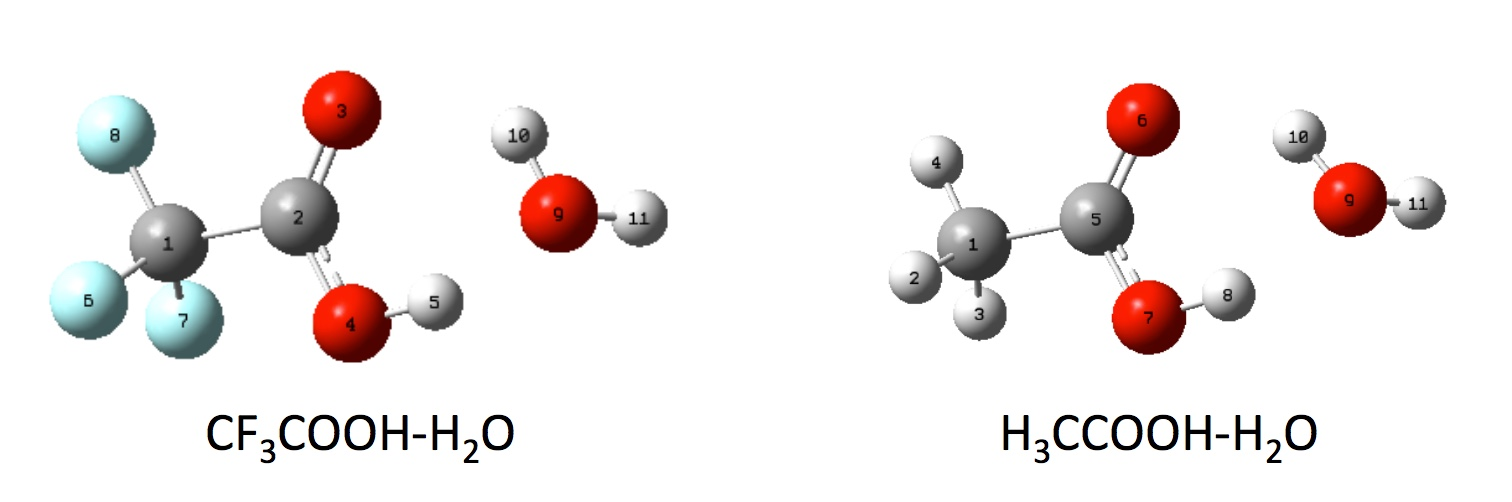
\includegraphics[scale=0.2]{acidos-h2o}
	\caption{Ácidos-$H_2O$}
\end{figure}
 Teniendo en cuenta el análisis NBO de dichas moléculas también comprobamos la mayor facilidad para romper el enlace O-H cuando se expone el ácido a la hidratación específica. En la molécula $H_3COOH$, los dos pares libres de electrones del átomo $O_7$ donan 5,69 y 44,35 Kcal/mol al enlace $C_5=O_6$ mientras que en la molécula de $H_3COOH-H_2O$, al formar un enlace de hidrógeno, los pares libres del $O_7$ donan 7,28 y 53,66 Kcal/mol, por lo que el enlace O-H se debilita, y en consecuencia aumenta la acidez de dicha molécula.
 La diferencia de acidez entre el $CF_3COOH$ y el $H_3COOH$ es de 24,53 Kcal/mol, hidratando los ácidos de forma específica ($CF_3COOH-H_2$ y $H_3COOH-H_2O$) la diferencia se reduce a 19,89 Kcal/mol. Esto lleva a pensar que el efecto del agua en ese punto, en el ácido trifluoretanoico, no es completo, puesto que el efecto inductivo del los tres halógenos compite con este. En el caso del ácido etanoico, al no tener efecto inductivo por parte de ninugn halógeno, el incremento de la acidez de dicho ácido es mayor al ser hidratado.
 Se ven algunas de las distancias de dichos ácidos en la tabla 3.14.
 \begin{table}[H]
 	\centering
 	\begin{tabular}{|c|c|c|c|c|c|c|}
 		\hline
 			 & d(C-F)	& d(O-H) & d(C=O) & & d(O-H) & d(C=O) \\ \hline
$CF_3COOH$ & 1,34 & 0,97 & 1,19 & $H_3CCOOH$ & 0,97 &1,21 \\ \hline $CF_3COOH-H_2O$	& 1,34 & 0,99 & 1,21 & $H_3CCOOH-H_2O$	& 0,99 &1,22 \\ \hline
 	\end{tabular}
 \caption{Distancias internucleares de interés de cada ácido en $\Armstrong$}
 \end{table}
Las d(C-F) son las mismas para las dos moléculas, en las demás distancias se observa una pequeña variación, haciendo uso del análisis NBO se ve que un par de electrones libre del $O_9$ de la molécula de $CF_3COOH-H_2O)$ actúa como donador de 24,26 Kcal/mol al enlace $O_4 - H_5$, actuando este último como aceptor. En contraste, en la molécula $H_3COOH-H_2O$, uno de los pares de electrones libres del $O_9$ dona 18,59 Kcal/mol de energía al enlace $O_7-H_8$. Y la energía donada por uno de los pares de electrones libres de los átomos de oxígeno $O_4 y O_7$ respectivamente, a los enlaces C=O correspondientes, es mayor en el ácido $CF_3COOH-H_2O$ que en el $H_3CCOOH-H_2O$.
